\section*{Problem 5}

Find the DTFT and the DFT of $x[n] = [1 -1]$. 
Sketch $X(\omega)$ for $-π < \omega < π$

\subsection*{Solution}

\begin{itemize}
\item FDTD

\begin{equation*}
\begin{aligned}
X(\omega)  &= e^{0} - e^{-j\omega} \\
&= e^{-j\omega/2}(e^{j\omega/2} - e^{-j\omega/2} \\
&= 2 j e^{-j\omega/2} \sin(\omega/2) \\
\end{aligned}
\end{equation*} 

\zcodemat{sources/c4p5.m}{Mlab for plotting $X(\omega)$}

\begin{figure}[H]
\caption{Plot for $X(\omega)$}
\centering
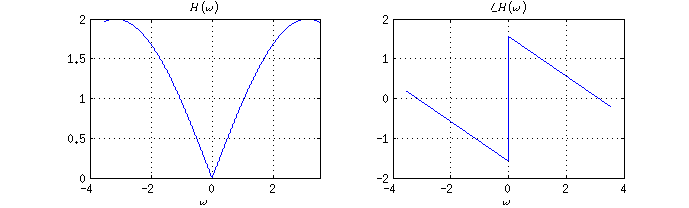
\includegraphics[width=0.8\textwidth]{figs/c4p5.png}
\label{fig:c4p5}
\end{figure} 

\item DFT

\begin{equation*}
\begin{aligned}
X_k &= e^{0} - e^{\frac{2 \pi k}{2} n}\\
&= 1 - e^{-j \pi k}\\
\\
X_0 &= 0 \\
X_1 &= 1-e^{-j \pi} = 2
\end{aligned}
\end{equation*} 
\end{itemize} 
